\begin{frame}{Continuous Distributions}
    So we’ve focused on cases where the outcome of a variable is discrete. 
    
    \vspace{12pt}Now we want to consider a context where the outcome is a continuous numerical variable.
\end{frame}

\begin{frame}{Continuous Distributions}
    \begin{center}
        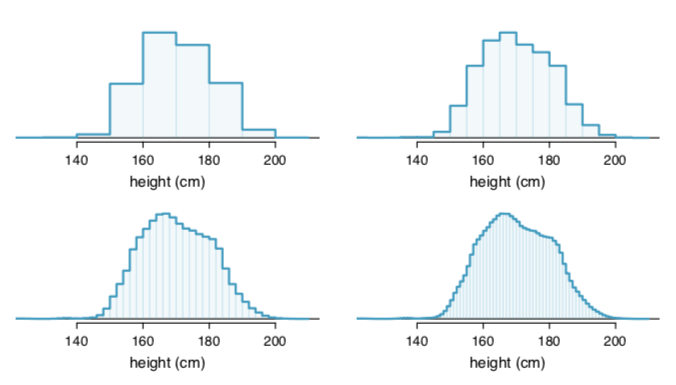
\includegraphics[scale=0.4]{images/hists.png}
    \end{center}
    
    \vspace{-20pt}\begin{itemize}
        \item These histograms are all of the same data.
        \item Varying bin widths allows us to make different interpretations of the data.
    \end{itemize}
\end{frame}

\begin{frame}{Continuous Distributions}
    \begin{center}
        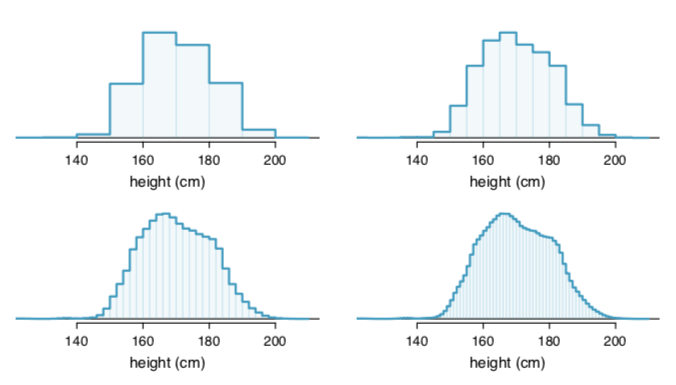
\includegraphics[scale=0.4]{images/hists.png}
    \end{center}
    
    \vspace{-20pt}\begin{itemize}
        \item By decreasing bin widths substantially, we "smooth out" the bumps in the histogram.
    \end{itemize}
\end{frame}

\begin{frame}{Example}
    \begin{center}
        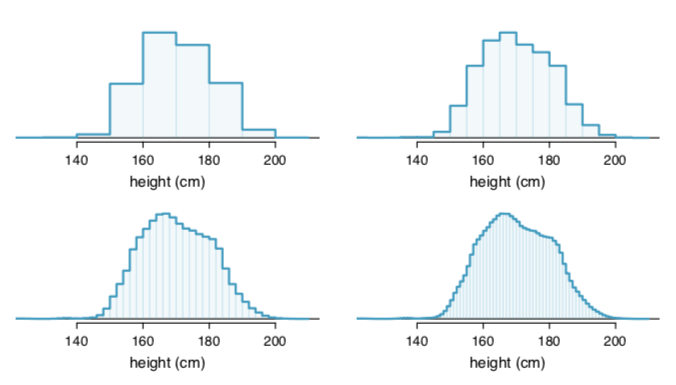
\includegraphics[scale=0.4]{images/hists.png}
    \end{center}
    What proportion of the sample is between 180 cm and 185 cm tall?
\end{frame}

\begin{frame}{Example}
    \begin{center}
        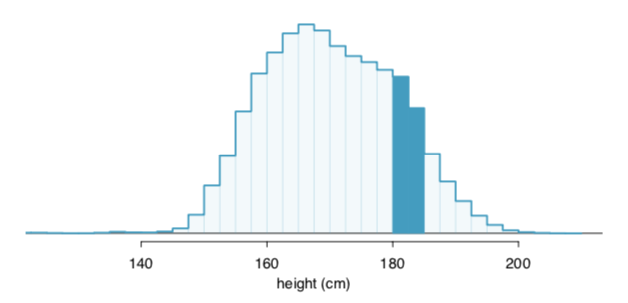
\includegraphics[scale=0.4]{images/heighthist.png}
    \end{center}
    \vspace{-12pt}To find the proportion of the sample between 180 and 185 cm,
    \begin{itemize}
        \item Add up the heights of the bins in the range 180 cm and 185 and divide by the sample size. 
    \end{itemize}
\end{frame}

\begin{frame}{Example}
    \begin{center}
        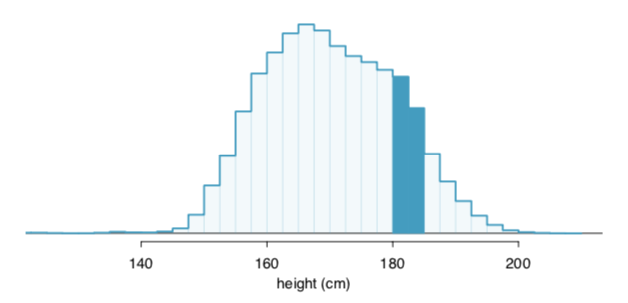
\includegraphics[scale=0.3]{images/heighthist.png}
    \end{center}
    \vspace{-20pt}\begin{itemize}
        \item This can be done with the two shaded bins. These have counts of 195,307 and 156,239 people:
        \[
            \frac{195307 + 156239}{3000000} = 0.1172 
        \]
        \item This fraction is the same as the proportion of the histogram’s area that falls in the range 180 to 185 cm.
    \end{itemize}
\end{frame}

\begin{frame}{Histograms to Continuous Distributions}
    \begin{center}
        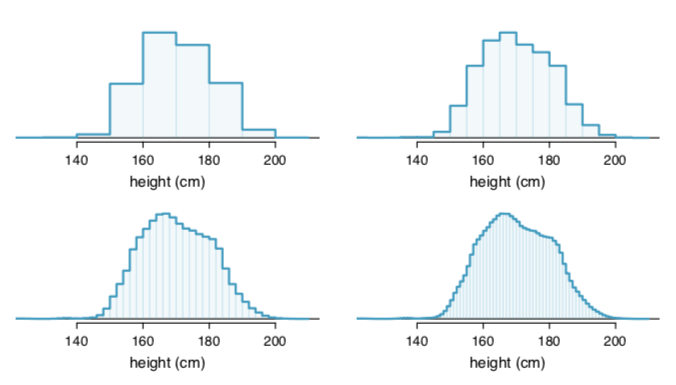
\includegraphics[scale=0.35]{images/hists.png}
    \end{center}
    \vspace{-12pt}\begin{itemize}
        \item Let's examine the transition from the boxy hollow histogram (top left)) to the much smoother one (bottom right).
        \item The last plot has so many bins that the histogram is starting to resemble a smooth curve.
    \end{itemize}
\end{frame}

\begin{frame}{Histograms to Continuous Distributions}
    \begin{center}
        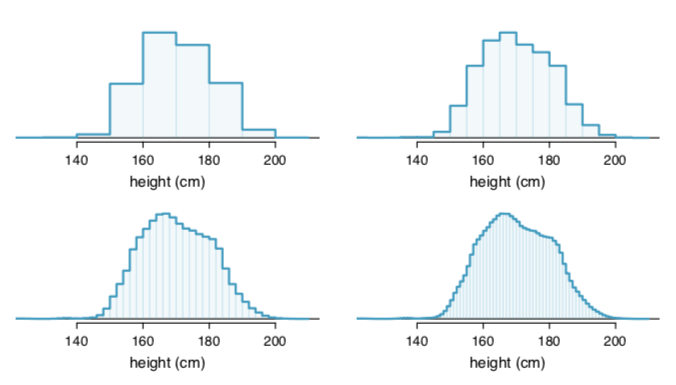
\includegraphics[scale=0.4]{images/hists.png}
    \end{center}
    \vspace{-12pt}Population height as a \textit{continuous} numerical variable might best be explained by a curve that represents the outline of extremely slim bins.
\end{frame}

\begin{frame}{Histograms to Continuous Distributions}
    \begin{itemize}
        \item This smooth curve represents a \textbf{probability density function}.
        \begin{itemize}
            \item There are also called a \textbf{density} or \textbf{distribution}.
        \end{itemize}
        \item A density has a special property: the total area under the density’s curve is 1.
    \end{itemize}
\end{frame}

\begin{frame}{Histograms to Continuous Distributions}
    \begin{center}
        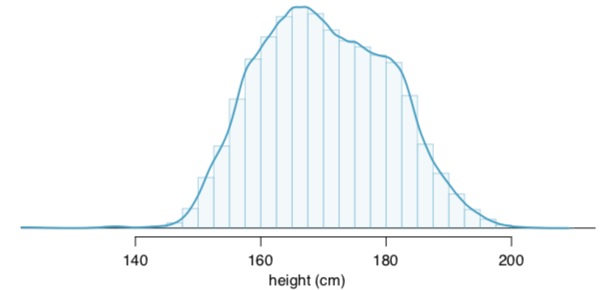
\includegraphics[scale=0.5]{images/heighthistdist.png}
    \end{center}
    Here, such a curve is shown overlaid on a histogram of the sample. 
\end{frame}

\begin{frame}{Probabilities from Continuous Distributions}
    We computed the proportion of individuals with heights 180 to 185 cm as 
    \[
        \frac{\text{number of people between 180 and 185cm}}{\text{total sample size}},
    \]
    the fraction of the histogram’s area in this region. 
\end{frame}

\begin{frame}{Probabilities from Continuous Distributions}
    \begin{center}
        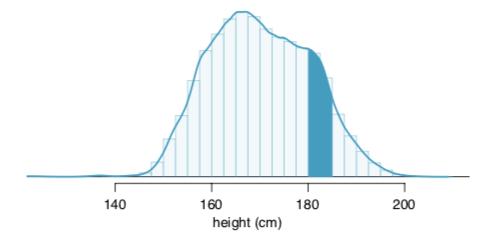
\includegraphics[scale=0.5]{images/shadedhistcurve.png}
    \end{center}
    We can also use the area in the shaded region under the curve to find a probability (using calculus or with the help of a computer):
    \[
        P(\text{height between }180\text{ and }185) = \text{area between }180\text{ and }185 = 0.1157
    \]
\end{frame}

\begin{frame}{Probabilities from Continuous Distributions}
    \begin{center}
        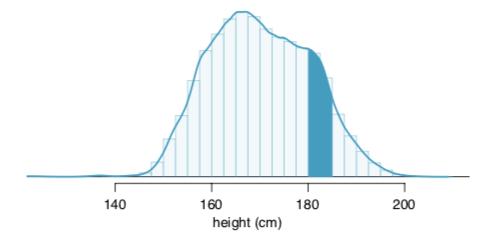
\includegraphics[scale=0.5]{images/shadedhistcurve.png}
    \end{center}

    The probability that a randomly selected person is between 180 and 185 cm is 0.1157. 
    
    \vspace{12pt}This is very close to the estimate from the previous example, when we used the histogram bins instead of the curve.
\end{frame}